% TMR cluster with one failed node -- include with % TMR cluster with one failed node -- include with % TMR cluster with one failed node -- include with % TMR cluster with one failed node -- include with \input{chapters/tmr_failure}
% Needs only TikZ + the positioning library (already loaded via forest in main.tex)
\begin{figure}[htbp]
  \centering
  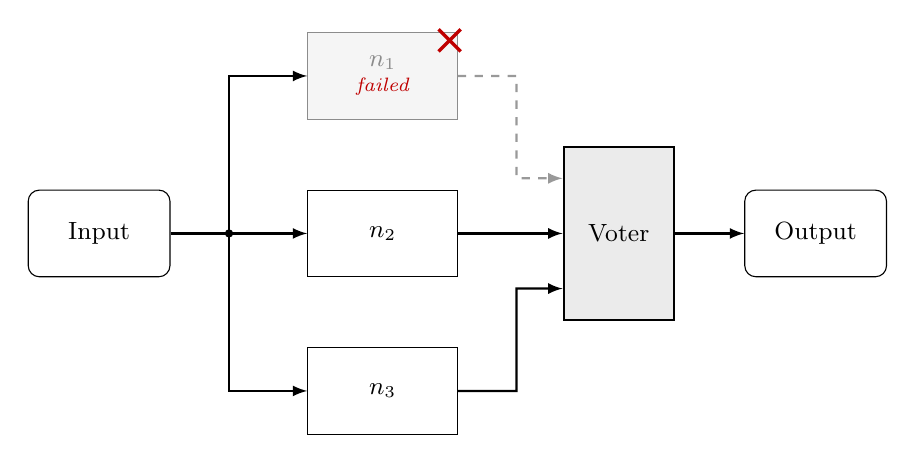
\begin{tikzpicture}[
      >=latex,
      font=\small,
      io/.style    ={draw, rounded corners=4pt, minimum width=1.8cm, minimum height=1.1cm},
      unit/.style  ={draw, minimum width=1.9cm, minimum height=1.1cm},
      failed/.style={unit, draw=black!45, text=black!45, fill=black!4},
      voter/.style ={draw, thick, fill=black!8, minimum width=1.4cm, minimum height=2.2cm,
                     align=center},
      wire/.style  ={draw, thick},
    ]
    % Nodes
    \node[io]   (in)  at (0,0)     {Input};
    \node[failed, align=center] (n1) at (3.6, 2.0)
      {$n_1$\\[-2pt]{\scriptsize\itshape\color{red!75!black} failed}};
    \node[unit] (n2)  at (3.6, 0)   {$n_2$};
    \node[unit] (n3)  at (3.6,-2.0) {$n_3$};
    \node[voter] (vot) at (6.6, 0)  {Voter};
    \node[io]   (out) at (9.1,0)   {Output};

    % Failure marker on n1: small red cross at the top-right corner
    \draw[red!75!black, very thick]
      ([shift={(-3pt,-3pt)}]n1.north east) ++(-4pt,-4pt) -- ++(8pt,8pt)
      ++(-8pt,0) -- ++(8pt,-8pt);

    % Fan-out from input to all three nodes
    \coordinate (split) at (1.65,0);
    \draw[wire] (in.east) -- (split);
    \draw[wire, ->] (split) |- (n1.west);
    \draw[wire, ->] (split) -- (n2.west);
    \draw[wire, ->] (split) |- (n3.west);
    \fill (split) circle (1.5pt);

    % Each node feeds its own voter input; n1 delivers no valid result
    \draw[wire, ->, dashed, black!40]
      (n1.east) -| (5.3, 0.7) -- ([yshift=0.7cm]vot.west);
    \draw[wire, ->] (n2.east) -- (vot.west);
    \draw[wire, ->]
      (n3.east) -| (5.3,-0.7) -- ([yshift=-0.7cm]vot.west);

    % Voter to output
    \draw[wire, ->] (vot.east) -- (out.west);
  \end{tikzpicture}

  \caption[TMR cluster with majority voter after failure of one node]{%
    Triple modular redundancy (TMR) cluster after the failure of node $n_1$.
    All three nodes receive the same input and feed their results to a
    majority voter. With $n_1$ failed, only $n_2$ and $n_3$ deliver results,
    so the cluster continues in degraded dual modular redundancy (DMR) mode:
    a disagreement between the two remaining nodes can still be detected,
    but no longer masked by a majority vote.}
  \label{fig:tmr-failure}
\end{figure}

% Needs only TikZ + the positioning library (already loaded via forest in main.tex)
\begin{figure}[htbp]
  \centering
  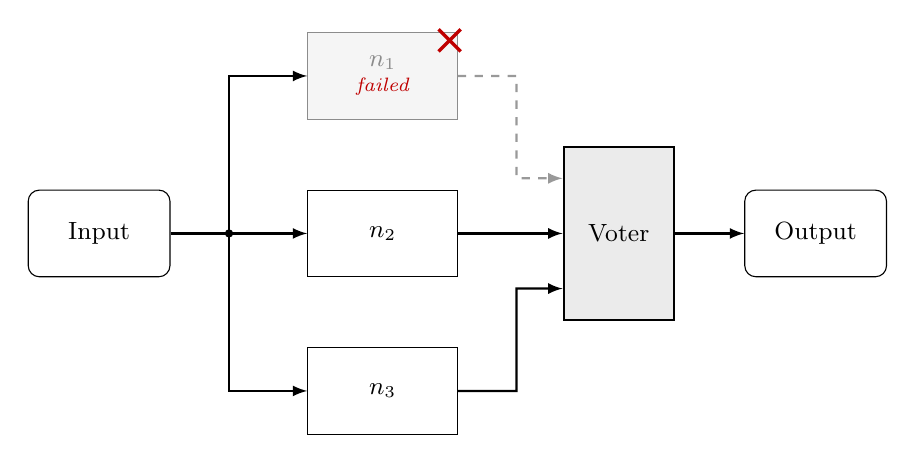
\begin{tikzpicture}[
      >=latex,
      font=\small,
      io/.style    ={draw, rounded corners=4pt, minimum width=1.8cm, minimum height=1.1cm},
      unit/.style  ={draw, minimum width=1.9cm, minimum height=1.1cm},
      failed/.style={unit, draw=black!45, text=black!45, fill=black!4},
      voter/.style ={draw, thick, fill=black!8, minimum width=1.4cm, minimum height=2.2cm,
                     align=center},
      wire/.style  ={draw, thick},
    ]
    % Nodes
    \node[io]   (in)  at (0,0)     {Input};
    \node[failed, align=center] (n1) at (3.6, 2.0)
      {$n_1$\\[-2pt]{\scriptsize\itshape\color{red!75!black} failed}};
    \node[unit] (n2)  at (3.6, 0)   {$n_2$};
    \node[unit] (n3)  at (3.6,-2.0) {$n_3$};
    \node[voter] (vot) at (6.6, 0)  {Voter};
    \node[io]   (out) at (9.1,0)   {Output};

    % Failure marker on n1: small red cross at the top-right corner
    \draw[red!75!black, very thick]
      ([shift={(-3pt,-3pt)}]n1.north east) ++(-4pt,-4pt) -- ++(8pt,8pt)
      ++(-8pt,0) -- ++(8pt,-8pt);

    % Fan-out from input to all three nodes
    \coordinate (split) at (1.65,0);
    \draw[wire] (in.east) -- (split);
    \draw[wire, ->] (split) |- (n1.west);
    \draw[wire, ->] (split) -- (n2.west);
    \draw[wire, ->] (split) |- (n3.west);
    \fill (split) circle (1.5pt);

    % Each node feeds its own voter input; n1 delivers no valid result
    \draw[wire, ->, dashed, black!40]
      (n1.east) -| (5.3, 0.7) -- ([yshift=0.7cm]vot.west);
    \draw[wire, ->] (n2.east) -- (vot.west);
    \draw[wire, ->]
      (n3.east) -| (5.3,-0.7) -- ([yshift=-0.7cm]vot.west);

    % Voter to output
    \draw[wire, ->] (vot.east) -- (out.west);
  \end{tikzpicture}

  \caption[TMR cluster with majority voter after failure of one node]{%
    Triple modular redundancy (TMR) cluster after the failure of node $n_1$.
    All three nodes receive the same input and feed their results to a
    majority voter. With $n_1$ failed, only $n_2$ and $n_3$ deliver results,
    so the cluster continues in degraded dual modular redundancy (DMR) mode:
    a disagreement between the two remaining nodes can still be detected,
    but no longer masked by a majority vote.}
  \label{fig:tmr-failure}
\end{figure}

% Needs only TikZ + the positioning library (already loaded via forest in main.tex)
\begin{figure}[htbp]
  \centering
  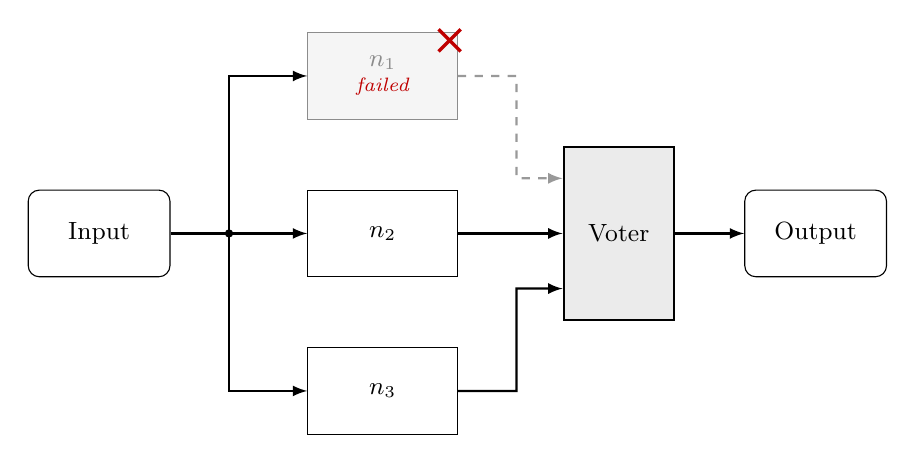
\begin{tikzpicture}[
      >=latex,
      font=\small,
      io/.style    ={draw, rounded corners=4pt, minimum width=1.8cm, minimum height=1.1cm},
      unit/.style  ={draw, minimum width=1.9cm, minimum height=1.1cm},
      failed/.style={unit, draw=black!45, text=black!45, fill=black!4},
      voter/.style ={draw, thick, fill=black!8, minimum width=1.4cm, minimum height=2.2cm,
                     align=center},
      wire/.style  ={draw, thick},
    ]
    % Nodes
    \node[io]   (in)  at (0,0)     {Input};
    \node[failed, align=center] (n1) at (3.6, 2.0)
      {$n_1$\\[-2pt]{\scriptsize\itshape\color{red!75!black} failed}};
    \node[unit] (n2)  at (3.6, 0)   {$n_2$};
    \node[unit] (n3)  at (3.6,-2.0) {$n_3$};
    \node[voter] (vot) at (6.6, 0)  {Voter};
    \node[io]   (out) at (9.1,0)   {Output};

    % Failure marker on n1: small red cross at the top-right corner
    \draw[red!75!black, very thick]
      ([shift={(-3pt,-3pt)}]n1.north east) ++(-4pt,-4pt) -- ++(8pt,8pt)
      ++(-8pt,0) -- ++(8pt,-8pt);

    % Fan-out from input to all three nodes
    \coordinate (split) at (1.65,0);
    \draw[wire] (in.east) -- (split);
    \draw[wire, ->] (split) |- (n1.west);
    \draw[wire, ->] (split) -- (n2.west);
    \draw[wire, ->] (split) |- (n3.west);
    \fill (split) circle (1.5pt);

    % Each node feeds its own voter input; n1 delivers no valid result
    \draw[wire, ->, dashed, black!40]
      (n1.east) -| (5.3, 0.7) -- ([yshift=0.7cm]vot.west);
    \draw[wire, ->] (n2.east) -- (vot.west);
    \draw[wire, ->]
      (n3.east) -| (5.3,-0.7) -- ([yshift=-0.7cm]vot.west);

    % Voter to output
    \draw[wire, ->] (vot.east) -- (out.west);
  \end{tikzpicture}

  \caption[TMR cluster with majority voter after failure of one node]{%
    Triple modular redundancy (TMR) cluster after the failure of node $n_1$.
    All three nodes receive the same input and feed their results to a
    majority voter. With $n_1$ failed, only $n_2$ and $n_3$ deliver results,
    so the cluster continues in degraded dual modular redundancy (DMR) mode:
    a disagreement between the two remaining nodes can still be detected,
    but no longer masked by a majority vote.}
  \label{fig:tmr-failure}
\end{figure}

% Needs only TikZ + the positioning library (already loaded via forest in main.tex)
\begin{figure}[htbp]
  \centering
  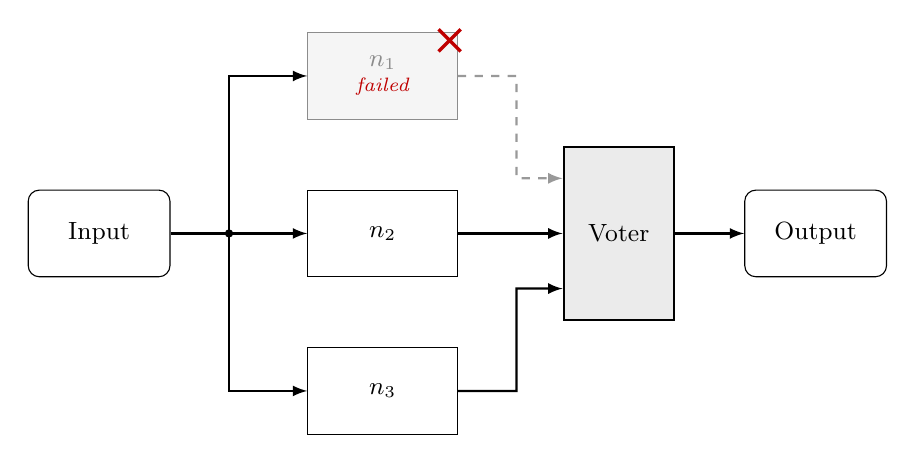
\begin{tikzpicture}[
      >=latex,
      font=\small,
      io/.style    ={draw, rounded corners=4pt, minimum width=1.8cm, minimum height=1.1cm},
      unit/.style  ={draw, minimum width=1.9cm, minimum height=1.1cm},
      failed/.style={unit, draw=black!45, text=black!45, fill=black!4},
      voter/.style ={draw, thick, fill=black!8, minimum width=1.4cm, minimum height=2.2cm,
                     align=center},
      wire/.style  ={draw, thick},
    ]
    % Nodes
    \node[io]   (in)  at (0,0)     {Input};
    \node[failed, align=center] (n1) at (3.6, 2.0)
      {$n_1$\\[-2pt]{\scriptsize\itshape\color{red!75!black} failed}};
    \node[unit] (n2)  at (3.6, 0)   {$n_2$};
    \node[unit] (n3)  at (3.6,-2.0) {$n_3$};
    \node[voter] (vot) at (6.6, 0)  {Voter};
    \node[io]   (out) at (9.1,0)   {Output};

    % Failure marker on n1: small red cross at the top-right corner
    \draw[red!75!black, very thick]
      ([shift={(-3pt,-3pt)}]n1.north east) ++(-4pt,-4pt) -- ++(8pt,8pt)
      ++(-8pt,0) -- ++(8pt,-8pt);

    % Fan-out from input to all three nodes
    \coordinate (split) at (1.65,0);
    \draw[wire] (in.east) -- (split);
    \draw[wire, ->] (split) |- (n1.west);
    \draw[wire, ->] (split) -- (n2.west);
    \draw[wire, ->] (split) |- (n3.west);
    \fill (split) circle (1.5pt);

    % Each node feeds its own voter input; n1 delivers no valid result
    \draw[wire, ->, dashed, black!40]
      (n1.east) -| (5.3, 0.7) -- ([yshift=0.7cm]vot.west);
    \draw[wire, ->] (n2.east) -- (vot.west);
    \draw[wire, ->]
      (n3.east) -| (5.3,-0.7) -- ([yshift=-0.7cm]vot.west);

    % Voter to output
    \draw[wire, ->] (vot.east) -- (out.west);
  \end{tikzpicture}

  \caption[TMR cluster with majority voter after failure of one node]{%
    Triple modular redundancy (TMR) cluster after the failure of node $n_1$.
    All three nodes receive the same input and feed their results to a
    majority voter. With $n_1$ failed, only $n_2$ and $n_3$ deliver results,
    so the cluster continues in degraded dual modular redundancy (DMR) mode:
    a disagreement between the two remaining nodes can still be detected,
    but no longer masked by a majority vote.}
  \label{fig:tmr-failure}
\end{figure}
